\documentclass[]{article}
\usepackage{amsmath, amsfonts}
\usepackage{enumitem}
\usepackage{fancyhdr}
\usepackage{geometry}
\usepackage{cancel}
\usepackage{graphicx}
\usepackage{color}
\usepackage{multirow}
\usepackage{float}
\usepackage{pgfplots}	% To draw charts directly in Latex
\usepackage{marvosym}	% For lightning symbol to denote contradiction
\usepackage{cleveref}	% For clever referencing :)

%TikZ package for drawing:
\usepackage{tikz}
%For calculation of coordinates:
\usetikzlibrary{calc}
\usetikzlibrary{positioning}

%opening
\title{Problem Set IV \\ \large Microeconomics II}
\author{Nurfatima Jandarova}
\date{\today}
\pagestyle{fancy}

\lhead{Microeconomics II, Problem Set IV}
\rhead{Nurfatima Jandarova}
\renewcommand{\headrulewidth}{0.4pt}
\fancyheadoffset{1 cm}

\geometry{a4paper, left=20mm, top=20mm, bottom = 20mm, headheight=20mm}

\sloppy
\definecolor{lightgray}{gray}{0.5}
\setlength{\parindent}{0pt}

\renewcommand{\arraystretch}{1.3}

\begin{document}

\maketitle

\subsection*{Exercise 1}

There are $n$ firms in a market for a homogeneous good. The demand function $F: \mathbb{R}_{+} \to \mathbb{R}_{+}, p \mapsto F(p)$, which satisfies the Law of Demand, i.e., it could be inverted $P(Q) = p \Leftrightarrow F(p) = Q$.Every firm $i$ displays a cost function $C_i: \mathbb{R}_{+} \to \mathbb{R}_{+}$, which is assumed increasing and strictly convex. 

\begin{enumerate}[label = \alph*)]
	\item Competitive market\\
	In a competitive environment, firms are price takers and hence each firm's objective is to maximize $\pi_i(q_i) = \bar{p}q_i - C_i(q_i)$. Firms choose their output $q_i^*$ such that $\bar{p} = C_i'(q_i^*)$.
	\item Cournot oligopoly\\
	In an oligopolistic market, firms internalize their effect on the market price. Therefore, now their objective is to maximize $\pi_i(q_i, q_{-i}) = P(\sum\limits_{i = 1}^nq_i)q_i - C_i(q_i)$ with respect to $q_i$. Assuming interior solution, the FOC is
	\begin{equation}
		\begin{split}
			C_i'(\hat{q}_i) - P(\hat{Q})& = P'(\hat{Q})\hat{q}_i \nonumber
		\end{split}
	\end{equation}
	Recall that the demand function satisfies the Law of Demand, i.e., $F'(p)<0$. Then, we also know that $P'(Q)<0$. Hence, the right-hand side is negative and at the optimum $C_i'(\hat{q}_i) - P(\hat{Q}) < 0$.
\end{enumerate}

Notice that the (type of) mark-up function $M(q_i, q_{-i}) = C_i'(q_i) - P(\sum\limits_{i = 1}^nq_i)$ is increasing in $q_i$:
\begin{equation}
\frac{\partial M(q_i, q_{-i})}{\partial q_i} = \underbrace{\frac{\partial^2C_i(q_i)}{\partial q_i^2}}_{\substack{>0\text{ since }C_i\\\text{ is strictly convex}}} - \underbrace{P'(Q)}_{<0} > 0 \nonumber
\end{equation}
Recall that in a competitive market $M(q_i, q_{-i})$ is equal to zero at equilibrium, while in Cournot oligopoly it is negative. Hence, it must be that $\hat{q}_i < q_i^* \Longrightarrow \hat{Q} < Q^*$.

\subsection*{Exercise 2}

Recall that we have 
\begin{itemize}
	\item a demand function $F: \mathbb{R}_{+}\to\mathbb{R}_{+}, p\mapsto F(p)$. By assumption, the demand function is affine, i.e., $F(p) = \tilde{a} - \tilde{b}p$. Since the demand function should also satisfy the Law of Demand, then we can invert the function and write $P(Q) = a - bQ \Leftrightarrow F(p) = Q$, where $a = \frac{\tilde{a}}{\tilde{b}}$, $b = \frac{1}{\tilde{b}}$, and $Q = \sum\limits_{i = 1}^nq_i$.
	\item a linear cost function (same for each firm, by assumption of the problem) $C:\mathbb{R}_{+}\to\mathbb{R}_{+}, q_i\mapsto C(q_i) = cq_i$. 
\end{itemize}

A Cournot-Nash equilibrium is a vector $q^* = (q_t^*, ..., q_n^*)$ such that each firm $i$ maximizes its profits:
\begin{equation}
	\begin{split}
		\max\limits_{q_i}\quad&\pi_i(q_i) = P(Q)q_i - C_i(q_i) = (a - b\sum\limits_{i = 1}^n q_i)q_i -  cq_i \\\nonumber
		\text{FOC: }&-bq_i^* + (a - bQ^*) - c = 0\\
		\text{Sum over all firms: }&n(a - c) = bQ^* + nbQ^* \\
		&Q^* = \frac{n}{1 + n}\frac{a - c}{b}
	\end{split}
\end{equation}
Since each firm has the same cost function and faces the same market demand, the optimal output supply is the same for all firms, i.e., $q_i = q_j, \forall i, j\in \{1, ..., n\}$ and $q_i^* = \frac{1}{n}Q^* = \frac{1}{1 + n}\frac{a - c}{b}, \forall i\in\{1, ..., n\}$. Then, $\pi_i(q_i) = \frac{1}{1 + n}\frac{a - c}{b}(a - \cancel{b}\frac{n}{1 + n}\frac{a - c}{\cancel{b}} - c) = \frac{1}{1 + n}\frac{a - c}{b}\frac{a - c}{1 + n} = \frac{1}{b}\begin{pmatrix}\frac{a - c}{1 + n}\end{pmatrix}^2$.

Next, observe that $\lim\limits_{n\to\infty} \frac{n}{1 + n} = 1$. Hence, as $n\to\infty$, NE allocation approaches competitive equilibrium allocation, derivation of which is shown below:
\begin{equation}
\begin{split}
\max\limits_{q_i}\quad&\pi_i(q_i) = \bar{p}q_i -  cq_i \\\nonumber
\text{FOC: }\bar{p}& = c\\
\text{Market clearing condition: }P(\sum\limits_{i = 1}^n\hat{q}_i(\bar{p}))& = a - b\sum\limits_{i = 1}^n\hat{q}_i(\bar{p}) = \bar{p} \\
\hat{Q}(\bar{p})& = \frac{a - \bar{p}}{b} = \frac{a - c}{b}\\
\text{and }\hat{q}_i(\bar{p})& = \frac{1}{n}\hat{Q}(\bar{p}) = \frac{1}{n}\frac{a - c}{b}
\end{split}
\end{equation}

\subsection*{Exercise 3}

\begin{itemize}
	\item[$\begin{bmatrix}\Rightarrow\end{bmatrix}$] Suppose we have a Bertrand-Nash equilibrium defined by $p^*$. Want to show that this implies ($\theta(p*) = c \wedge \#\{j\in N: p_j^* = \theta(p^*)\}\geq2$). This is equivalent to showing that $\theta(p*) \neq c \vee \#\{j\in N: p_j^* = \theta(p^*)\}<2 \Longrightarrow p^*$ is not NE.
	\begin{itemize}
		\item[] $\theta(p^*) < c$: then $\exists i\in N: p_i^* = \theta(p^*) < c$. Consequently, this firm's profit is given by $\pi_i(p^*) = \underset{<0}{(\theta(p^*) - c)}\underset{>0}{\frac{F(\theta(p^*))}{\eta(p^*)}} < 0$. Consider a deviation to $\hat{p}_i > \theta(p^*)$. Then, $\pi_i(\hat{p}_i, p_{-i}^*) = 0$, which implies that $\hat{p}_i$ constitutes a profitable deviation. But it contradicts the fact that $p^*$ is NE.
		
		\item[] $\theta(p^*) > c$: i.e., $\exists j\in N: p_j^* = \theta(p^*) > c$. Then, there exists firm $j$ and $\varepsilon > 0$ small enough such that $\hat{p}_j = \theta(p^*) - \varepsilon\in(c, \theta(p^*))$ and
		\begin{equation}
			\pi_j(\hat{p}_j, p_{-j}^*) = (\theta(p^*) - \varepsilon - c)F(\theta(p^*) - \varepsilon) > (\theta(p^*) - c)\frac{F(\theta(p^*))}{\eta(p^*)} = \pi_j(p^*) \nonumber
		\end{equation}
		This again contradicts the assumption in the very beginning that $p^*$ is a NE.
		\item[]$\#\{j\in N: p_j^* = \theta(p^*)\}<2$: i.e., there is one firm $j$, which charges $p_j^* = \theta(p^*)$. Define $p_i^*$ as a second lowest price charged by some firm $i$. Then, $\exists\varepsilon>0$ such that $\hat{p}_j = \theta(p^*) + \varepsilon \in (\theta(p^*), p_i^*)$ and
		\begin{equation}
			\pi_j(\hat{p}_j, p_{-j}^*) = (\theta(p^*) + \varepsilon - c)F(\theta(p^*) + \varepsilon) > (\theta(p^*) - c)F(\theta(p^*)) \nonumber
		\end{equation}
		In other words, by increasing the price infinitesimally the firm $j$ could still absorb the whole market demand at a slightly higher mark-up, i.e., a profitable deviation. \Lightning
	\end{itemize}
	Thus, $(p^* \text{ is Bertrand-Nash equilibrium }) \Longrightarrow (\theta(p*) = c \wedge \#\{j\in N: p_j^* = \theta(p^*)\}\geq2)$.
	
	\item[$\begin{bmatrix}\Leftarrow\end{bmatrix}$] Take firm $j$ such that $p_j^* = \theta(p^*)$ and consider a unilateral deviation to $\tilde{p}_j > \theta(p^*)$. Then, $\#\{j\in N: p_j^* = \theta(p^*)\}\geq1$ and by deviating to $\tilde{p}_j$, firm $j$ reduces its profit to 0. Consider another deviation of this firm to $\tilde{p}_j < \theta(p^*) = c$. Then, $\pi_j(\tilde{p}_j, p_{-j}^*) = (\tilde{p}_j - c)F(\tilde{p}_j) < 0$, not a profitable deviation. Similar reasoning also helps to eliminate deviation of any other firm to a price lower than marginal cost. Hence, any price system deviation away from the one characterized by $(\theta(p*) = c \wedge \#\{j\in N: p_j^* = \theta(p^*)\}\geq2)$ cannot constitute a profitable deviation. Therefore, any price system $p^*$ that satisfies $(\theta(p*) = c \wedge \#\{j\in N: p_j^* = \theta(p^*)\}\geq2)$ is a Bertrand-Nash equilibrium.
\end{itemize}

\subsection*{Exercise 4}

Define the strategy profile space $S = \{(C, C), (C, F), (F, C), (F, F)\}$ and probability distribution over the strategy profiles $q = \{p_1, p_2, p_3, p_4\}$. Then, the expected payoffs of the players are
\begin{equation}
	\begin{split}
		\pi_1(q) = p_12 + p_20 + p_30 + p_45 = 2p_1 + 5p_4 \\ \nonumber
		\pi_2(q) = p_15 + p_20 + p_30 + p_42 = 5p_1 + 2p_4
	\end{split}
\end{equation}

Player 1 gets recommendation to play $C$ with probability $p_1 + p_2$ and to play $F$ with probability $p_3 + p_4$. Then, given that first player gets recommendation to play $C$, probability of the second player to be advised to play $C$ is $\frac{p_1}{p_1 + p_2}$. Similarly, probability of the second player to be recommended with action $F$ given the first player was recommended to play $F$ is $\frac{p_4}{p_3 + p_4}$.

\begin{enumerate}[label = \roman*)]
	\item According to the definition, $q$ is a correlated equilibrium if $\forall i\in\{1, 2\}$ and $\forall \eta_i:\Sigma_i\to\Sigma_i$
	\begin{equation}
		\sum\limits_{\sigma\in\Sigma}q(\sigma)\pi_i(\sigma)\geq\sum\limits_{\sigma\in\Sigma}q(\sigma)\pi_i(\eta_i(\sigma_i), \sigma_{-i}) \nonumber
	\end{equation}
	Applied to this example, the above is equivalent to the following set of inequalities
	\begin{equation}\label{correq}
		\begin{split}
			\begin{cases}
			2\frac{p_1}{p_1 + p_2} + 0\frac{p_2}{p_1 + p_2} \geq 0\frac{p_1}{p_1 + p_2} + 5\frac{p_2}{p_1 + p_2} \\
			0\frac{p_3}{p_3 + p_4} + 5\frac{p_4}{p_3 + p_4} \geq 2\frac{p_3}{p_3 + p_4} + 0\frac{p_4}{p_3 + p_4} \\
			5\frac{p_1}{p_1 + p_3} + 0\frac{p_3}{p_1 + p_3} \geq 0\frac{p_1}{p_1 + p_3} + 2\frac{p_3}{p_1 + p_3} \\
			0\frac{p_2}{p_2 + p_4} + 2\frac{p_4}{p_2 + p_4} \geq 5\frac{p_2}{p_2 + p_4} + 0\frac{p_4}{p_2 + p_4}
			\end{cases} \Longrightarrow \begin{cases}
			p_1 \geq \frac{5}{2}p_2 \\
			p_4 \geq \frac{2}{5}p_3 \\
			p_1 \geq \frac{2}{5}p_3 \\
			p_4 \geq \frac{5}{2}p_2
			\end{cases}
		\end{split}
	\end{equation}
	We are also asked to find a correlated equilibrium such that it maximizes the expected payoff of player 1
	\begin{equation}
		\max\limits_{q} 2p_1 + 5p_4 \nonumber
	\end{equation}
	It is clear from above that the maximum possible payoff for player 1 is attained when $p_4 = 1$. Moreover, $q = \{0, 0, 0, 1\}$ satisfies the set of inequalities in \eqref{correq}. Hence, $q = \{0, 0, 0, 1\}$ is libertarian equilibrium for player 1.
	
	\item To find the libertarian equilibrium for player 2, have to find $q$ such that satisfies \eqref{correq} and 
	\begin{equation}
		\max\limits_{q} 5p_1 + 2p_4 \nonumber
	\end{equation}
	Again, if $p_1 = 1$ results in a highest possible payoff for the second player and
	\begin{equation}
		\begin{split}
			\begin{cases}
				1 \geq 0 \\
				0 \geq 0 \\
				1 \geq 0 \\
				0 \geq 0
			\end{cases} \nonumber
		\end{split}
	\end{equation}
	Therefore, $q = \{1, 0, 0, 0\}$ is a libertarian equilibrium for player 2.
	
	\item Now $q$ should satisfy \eqref{correq} and 
	\begin{equation}
		\max\limits_{q} 2p_1 + 5p_4 + 5p_1 + 2p_4 = \max\limits_{q}7(p_1 + p_4) \nonumber
	\end{equation}
	It is again possible to see that the maximum is attained when $p_1 + p_4 = 1 \Longrightarrow p_4 = 1 - p_1$. Let's check if \eqref{correq} is satisfied:
	\begin{equation}
		\begin{split}
			\begin{cases}
				p_1 \geq 0 \\
				1 - p_1 \geq 0 \\
				p_1 \geq 0 \\
				1 - p_1 \geq 0
			\end{cases} \nonumber
		\end{split}
	\end{equation}
	Therefore, all distributions over strategy profiles $q = \{p_1, 0, 0, 1 - p_1\}$, where $p_1\in[0, 1]$, define a set of utilitarian equilibria.
	
	\item I'm not sure if I understood the concept of egalitarian equilibrium, but after some googling and staring at the definition in the problem set, I think it is the probability distribution that satisfies \eqref{correq} and 
	\begin{equation}
		\max\limits_{q}\min\{2p_1 + 5p_4, 5p_1 + 2p_4\}\nonumber
	\end{equation}
	Graphically, the maximization problem looks like in \Cref{fig:egalitarian}
	
	\begin{figure}[h]
		\centering
		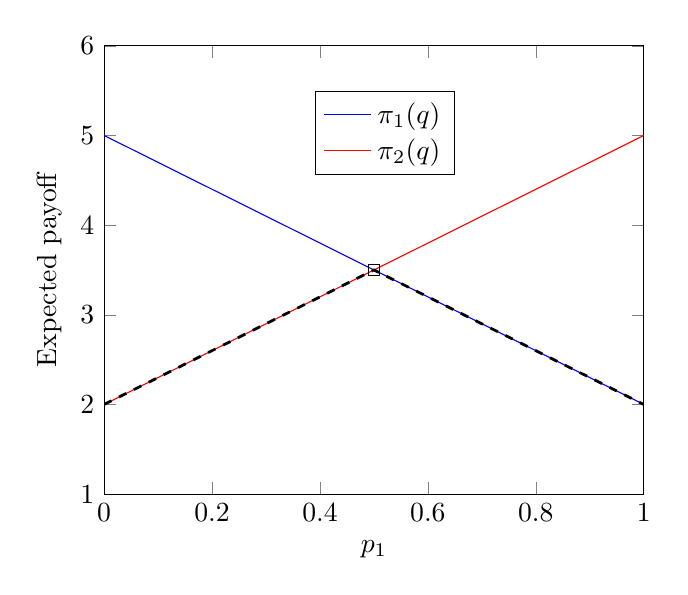
\begin{tikzpicture}
		\begin{axis}[
		xlabel={$p_1$},
		ylabel={Expected payoff},
		xmin=0, xmax=1,
		ymin=1, ymax=6,
		legend style={at={(0.65,0.9)},anchor=north east},
		ymajorgrids=false,
		]
		
		% Expected payoff of the first player
		\addplot[color = blue, ]
		coordinates {(0,5)(1,2)};
		
		% Expected payoff of the second player
		\addplot[color=red, ]
		coordinates {(0,2)(1,5)};
		
		% Minimum expected payoff
		\addplot[color=black, line width = 1.0, dashed]
		coordinates {(0, 2)(0.5,7/2)(1,2)};
		
		% Egalitarian equilibrium
		\addplot[only marks, mark=square]
		coordinates {(0.5, 7/2)};
		
		\legend{$\pi_1(q)$, $\pi_2(q)$}
		\end{axis}
		\end{tikzpicture}
		\caption{Egalitarian equilibrium}
		\label{fig:egalitarian}
	\end{figure}
	Hence, the solution is found at the point where the two expected payoffs are equal:
	\begin{equation}
		2p_1 + 5p_4 = 5p_1 + 2p_4 \Longrightarrow p_1 = p_4 \nonumber
	\end{equation}
	For these to be probability measures we also need them to add up to 1. So, $p_4 = 1 - p_1 \Longrightarrow 2p_1 = 1 \Longrightarrow p_1 = p_4 = \frac{1}{2}$. Notice that $q = (\frac{1}{2}, 0, 0, \frac{1}{2})$ does indeed satisfy conditions for correlated equilibria given in \eqref{correq}, and hence is an egalitarian equilibrium.
	
	\item \Cref{fig:setattpayoff} depicts the set of two Nash equilibria in pure strategies (which are also the respective libertarian equilibria for player 1 LE$_1$ and for player 2 LE$_2$), Nash equilibrium in mixed strategies (ME), set of utilitarian equilibria (UE) and egalitarian equilibrium (EE).
	\begin{figure}[h]
		\centering
		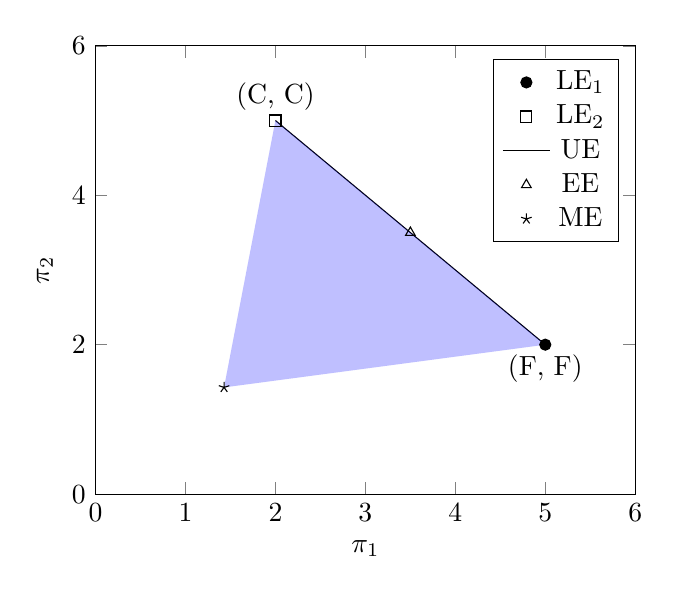
\begin{tikzpicture}
		\begin{axis}[
		xlabel={$\pi_1$},
		ylabel={$\pi_2$},
		xmin=0, xmax=6,
		ymin=0, ymax=6,
		legend pos = north east,
		ymajorgrids=false,
		]
		
		% Libertarian equilibrium for first player
		\addplot[only marks, mark = *, nodes near coords = {(F, F)}, every node near coord/.append style={yshift=-0.6cm}, ]
		coordinates {(5,2)};
		
		% Libertarian equilibrium for second player
		\addplot[only marks, mark = square, nodes near coords = {(C, C)}, ]
		coordinates {(2,5)};
		
		% Utilitarian equilibrium
		\addplot[ ]
		coordinates {(5, 2)(2, 5)};
		
		% Egalitarian equilibrium
		\addplot[only marks, mark = triangle, ]
		coordinates {(7/2, 7/2)};
		
		% Mixed equilibrium
		\addplot[only marks, mark = star,]
		coordinates {(10/7, 10/7)};
		
		% Set of possible correlated equilibria under pulic signal
		\addplot[patch, color = blue, opacity = 0.01, fill opacity = 0.25, faceted color = none, ]
		coordinates {(10/7, 10/7)(2, 5)(5, 2)};
		
		\legend{LE$_1$, LE$_2$, UE, EE, ME}
		\end{axis}
		\end{tikzpicture}
		\caption{The set of attainable payoffs}
		\label{fig:setattpayoff}
	\end{figure}

	Recall that any point within the shaded area could be obtained as a correlated equilibrium with public information about the outcome of a stochastic device. Then, notice that the line connecting two NE in pure strategies also defines the set of Pareto efficient outcomes under public signal: it is not possible to achieve a higher payoff for one player without making the other worse off. Thus, any utilitarian equilibrium, including the two libertarian and egalitarian equilibria, is a Pareto efficient outcome. 
\end{enumerate}
\end{document}
